% Created 2023-03-23 Thu 18:06
% Intended LaTeX compiler: lualatex
\documentclass[11pt]{article}
\usepackage[margin=0.5in]{geometry}
\usepackage{syntax}
\usepackage{pdfpages}
\usepackage{tcolorbox}
\usepackage{etoolbox}
\usepackage{environ}
\usepackage[ruled]{algorithm2e}
\let\oldtabular\tabular
\let\oldendtabular\endtabular
\NewEnviron{tabular2}[1]{\tcbox[left=0mm, right=0mm, top=0mm, bottom=0mm]{\oldtabular{#1}\BODY\oldendtabular}}
\BeforeBeginEnvironment{minted}{\begin{tcolorbox}}%
\AfterEndEnvironment{minted}{\end{tcolorbox}}
\BeforeBeginEnvironment{verbatim}{\begin{tcolorbox}}%
\AfterEndEnvironment{verbatim}{\end{tcolorbox}}
\usepackage{graphicx}
\usepackage{longtable}
\usepackage{wrapfig}
\usepackage{rotating}
\usepackage[normalem]{ulem}
\usepackage{amsmath}
\usepackage{amssymb}
\usepackage{capt-of}
\usepackage{hyperref}
\usepackage{minted}
\usepackage{physics}
\author{David Lewis}
\date{}
\title{lec20}
\hypersetup{
 pdfauthor={David Lewis},
 pdftitle={lec20},
 pdfkeywords={},
 pdfsubject={},
 pdfcreator={Emacs 30.0.50 (Org mode 9.6.1)}, 
 pdflang={English}}
\begin{document}

\maketitle

\section*{1.}
\label{sec:orgfee0ee3}
\subsection*{a.}
\label{sec:org1f8298c}

\begin{center}
\begin{tabular2}{l|rrrr}
I & B & C & D & E\\[0pt]
\hline
A & 9 & 1 & 4 & 6\\[0pt]
B &  & 4 & 1 & 4\\[0pt]
C &  &  & 4 & 4\\[0pt]
D &  &  &  & 4\\[0pt]
\end{tabular2}
\end{center}

A merged with C

\begin{center}
\begin{tabular2}{l|lrr}
 & B & D & E\\[0pt]
\hline
AC & 13/2 & 5/2 & 5\\[0pt]
B &  & 1 & 4\\[0pt]
D &  &  & 4\\[0pt]
\end{tabular2}
\end{center}

B merged with D
\begin{center}
\begin{tabular2}{lrr}
 & BD & E\\[0pt]
\hline
AC & 9 & 5\\[0pt]
BD &  & 4\\[0pt]
\end{tabular2}
\end{center}

BD merged with E
\begin{center}
\begin{tabular2}{lr}
 & BDE\\[0pt]
\hline
AC & 7\\[0pt]
\end{tabular2}
\end{center}

\begin{center}
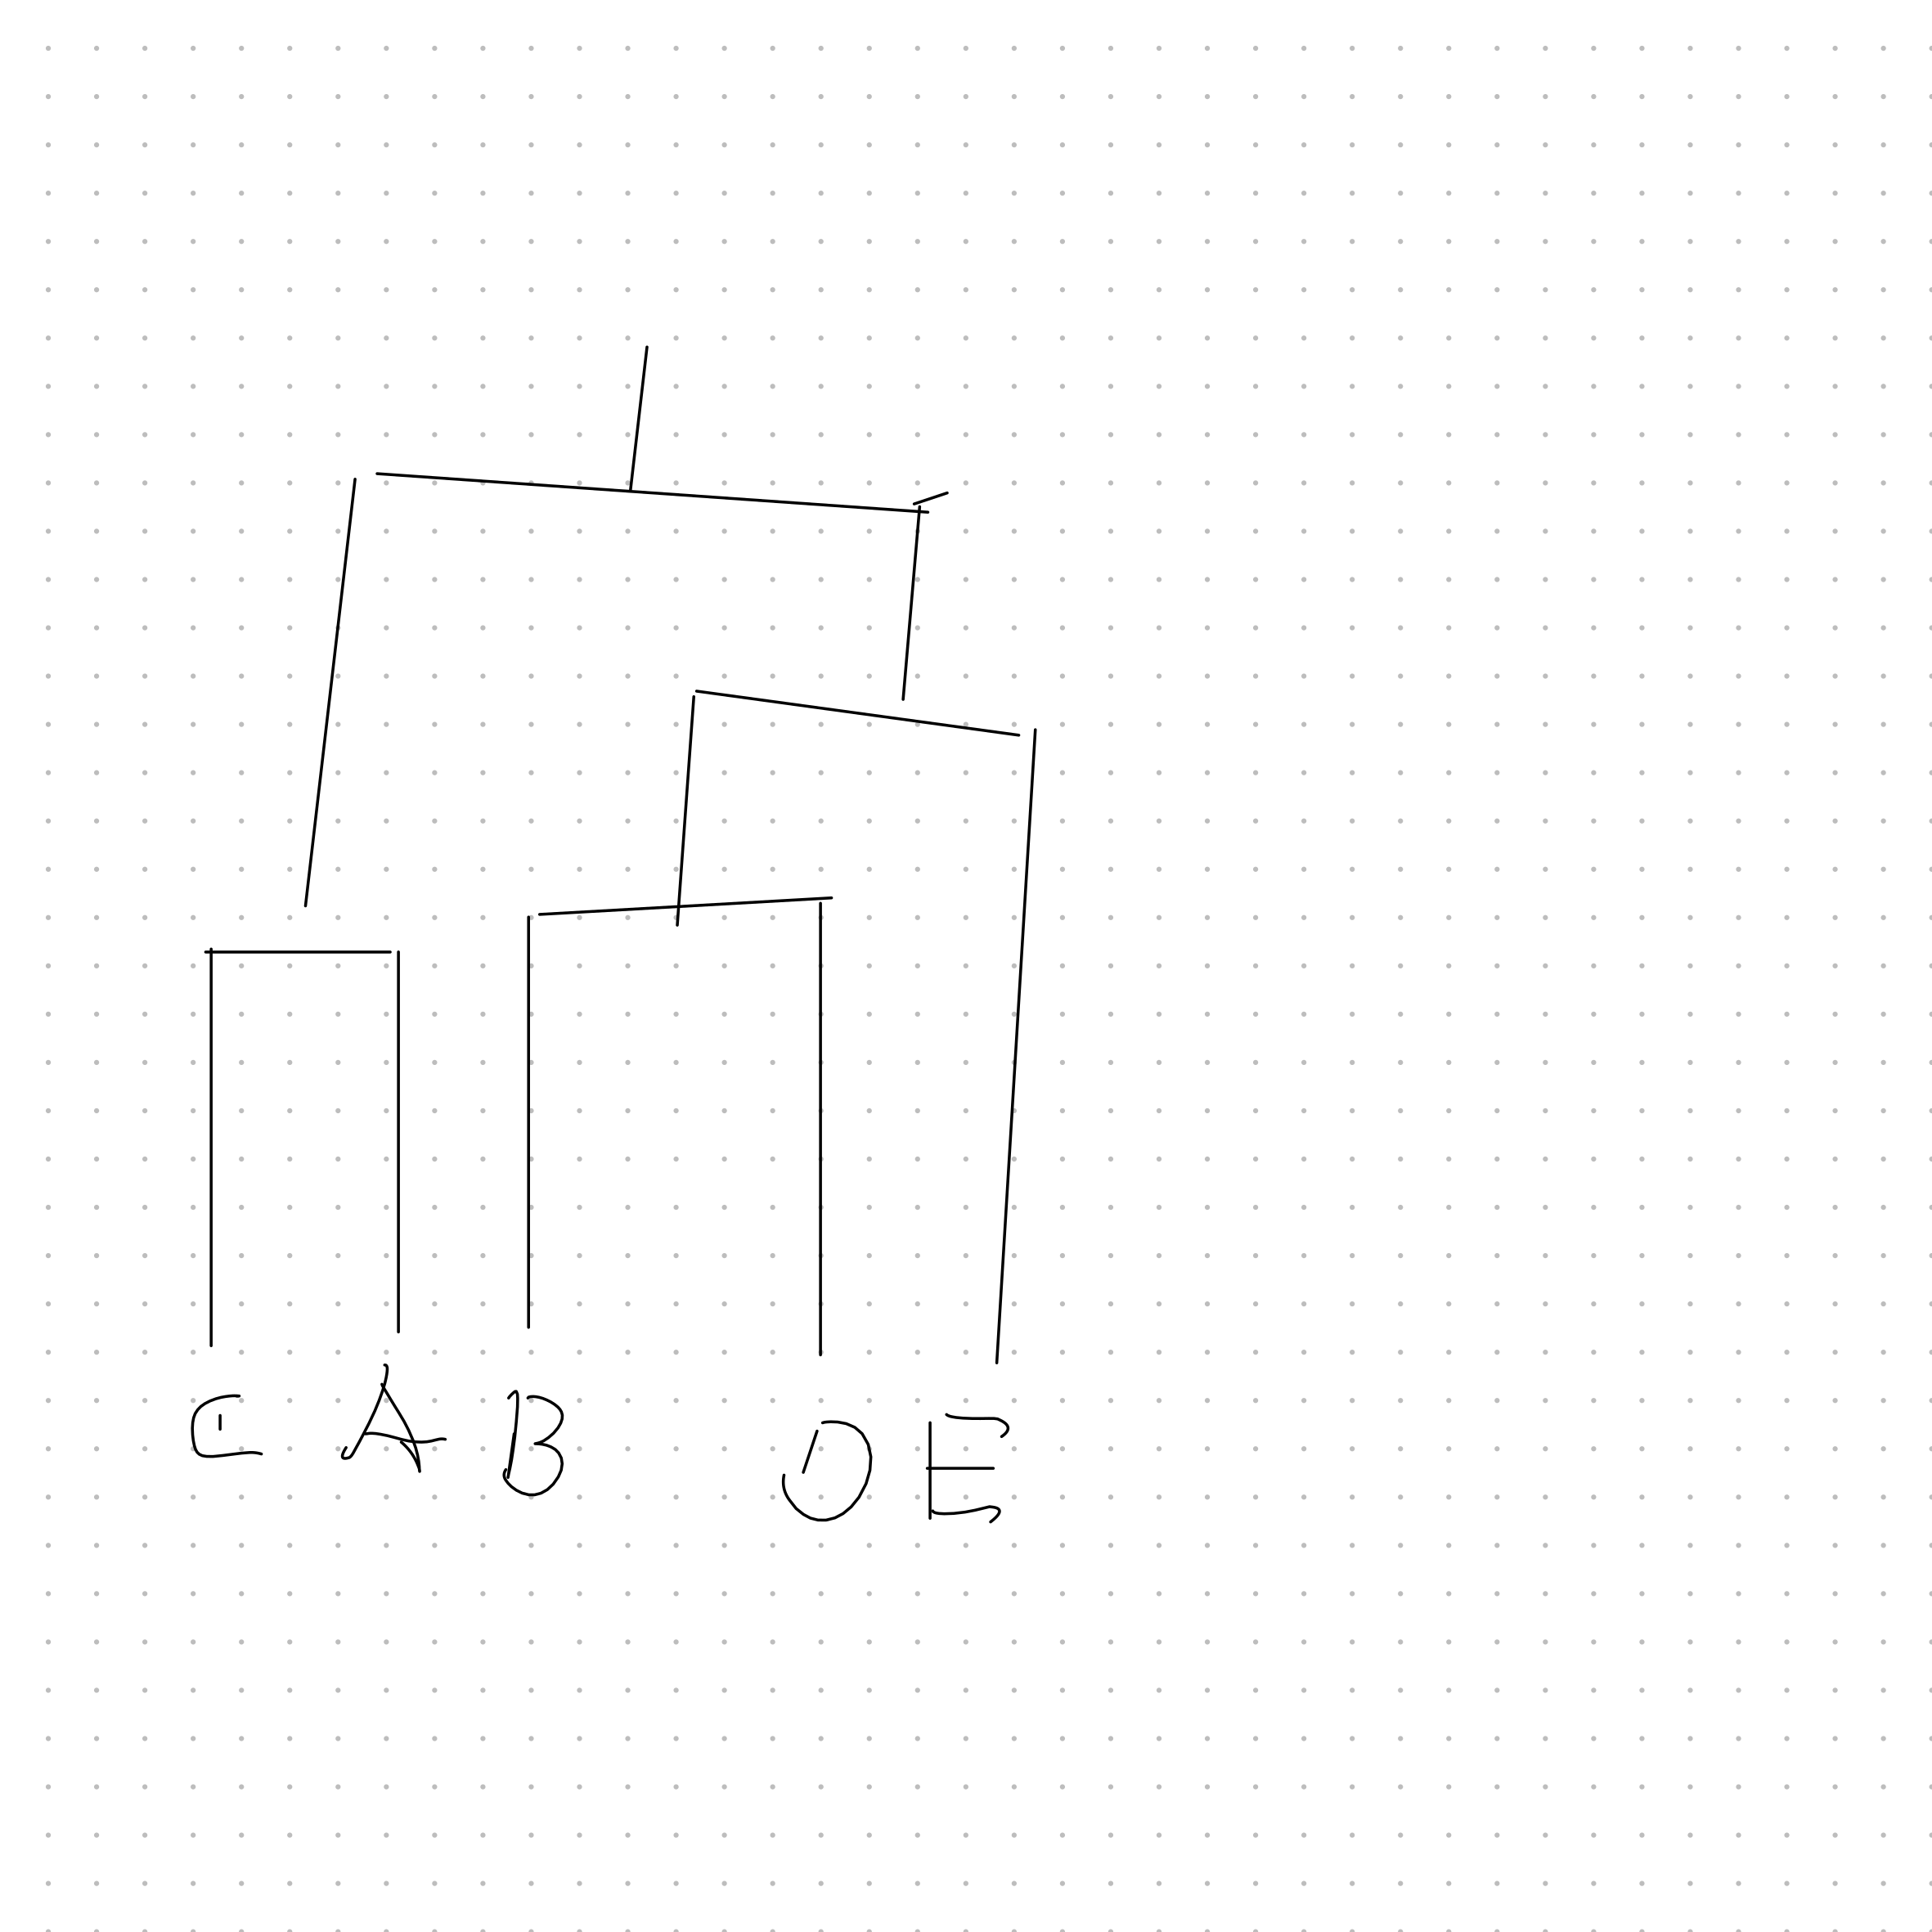
\includegraphics[width=0.7\textwidth]{1.png}
\end{center}

Reformat table to check with python
\begin{table}[htbp]
\label{d}
\centering
\begin{tabular2}{lr|rrrr}
I & A & B & C & D & E\\[0pt]
\hline
A & 0 & 9 & 1 & 4 & 6\\[0pt]
B & 9 & 0 & 4 & 1 & 4\\[0pt]
C & 1 & 4 & 0 & 4 & 4\\[0pt]
D & 4 & 1 & 4 & 0 & 4\\[0pt]
E & 6 & 4 & 4 & 4 & 0\\[0pt]
\end{tabular2}
\end{table}

\begin{minted}[fontsize=\scriptsize]{python}
import scipy.cluster.hierarchy as shc
from scipy.spatial.distance import squareform, pdist
import pandas as pd
import matplotlib.pyplot as plt
from scipy.spatial.distance import squareform, pdist

D = pd.DataFrame(D)
D.columns = ["I", "A", "B", "C", "D", "E"]
D = D.set_index("I")

D = D.drop("/")
fig, ax = plt.subplots()
dend = shc.dendrogram(shc.linkage(squareform(D), method='average'), labels=D.index, ax=ax)
plt.show()
\end{minted}

\begin{center}
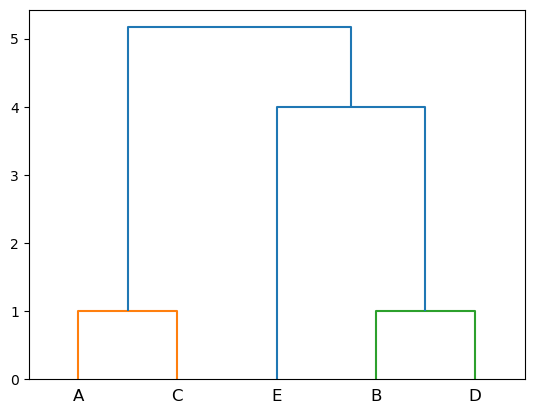
\includegraphics[width=0.7\textwidth]{./.ob-jupyter/3a11fd48cbe6a3069ecc828cee581839012b140d.png}
\end{center}

\subsection*{b.}
\label{sec:org7d1c34b}

\begin{itemize}
\item \(d(ij)k = \alpha_id_{ik} + \alpha_jd_{jk} + \beta d_{ij} + \gamma|d_{ik} - d_{jk}\)
\item \(d(ij)k = \frac{n_i}{n_i + n_j} d_{ik} + \frac{n_j}{n_i + n_j} d_{jk} + 0\)
\item \(\sum_{x \in C_i \cup C_j}a = \sum_{x \in C_i}a + \sum_{x \in C_j}a\)
\item \(\delta(C_i\cup C_j, C_k) = \frac{\left[\sum \limits_{x \in C_i} \sum \limits_{y \in C_k} d(x, y)\right] +
  \left[\sum \limits_{x \in C_j} \sum \limits_{y \in C_k} d(x, y)\right]}{(n_i + n_j)n_k}\)
\item \(d_{ik} = \frac{\sum_{x \in C_i}\sum_{y \in C_k}}{n_in_k}\)
\item 

\item \(\sum _{x \in C_i} \sum _{x \in C_k} d(x, y) = n_id_{ik}/n_k\)
\item \(\delta(C_i \cup C_j, C_k) = \frac{n_id_{ik} + n_jd_{jk}}{(n_i + n_j)}\)
\item \(d(ij)k = \delta(C_i \cup C_j, C_k) =  \frac{n_i}{n_i + n_j} d_{ik} + \frac{n_j}{n_i + n_j} d_{jk}\)
\end{itemize}
\section*{2.}
\label{sec:org5223179}
\subsection*{a.}
\label{sec:orgdeacc21}
Neighbors are within \(\epsilon\) of each point
\begin{minted}[fontsize=\scriptsize]{python}
D = [1, 3, 4, 5, 8, 9, 10, 11, 20]
N = []
e = 2

for point in D:
    n = []
    for p in range(point-2, point+e+1):
        if p in D and p is not point:
            n.append(p)
    N.append(n)

D = list(zip(D, N))
D
\end{minted}

\begin{center}
\begin{tabular2}{rl}
1 & (3)\\[0pt]
3 & (1 4 5)\\[0pt]
4 & (3 5)\\[0pt]
5 & (3 4)\\[0pt]
8 & (9 10)\\[0pt]
9 & (8 10 11)\\[0pt]
10 & (8 9 11)\\[0pt]
11 & (9 10)\\[0pt]
20 & nil\\[0pt]
\end{tabular2}
\end{center}
\subsection*{b.}
\label{sec:org576c6cc}
A point is a core point if it has at least min points
\begin{minted}[fontsize=\scriptsize]{python}
min_points = 3
C = []
for point, neighbors in D:
    if len(neighbors) >= min_points:
        C.append(point)
C
\end{minted}

\begin{center}
\begin{tabular2}{rrr}
3 & 9 & 10\\[0pt]
\end{tabular2}
\end{center}
\subsection*{c.}
\label{sec:orgc0dfa39}
A point is a border point if it is within \(\epsilon\) of a core point (a neighbor) and
is not also a core point
\begin{minted}[fontsize=\scriptsize]{python}
B = []
for point, neighbors in D:
    if point in C:
        B += [n for n in neighbors if n not in C]
B = set(B)
B
\end{minted}

\begin{center}
\begin{tabular2}{rrrrr}
1 & 4 & 5 & 8 & 11\\[0pt]
\end{tabular2}
\end{center}
\subsection*{d.}
\label{sec:org44c4843}
A point is a noise point if is not a border point or a core point.
\begin{minted}[fontsize=\scriptsize]{python}
# * operator unpacks list
[i for i in list(zip(*D))[0] if i not in B and i not in C]
\end{minted}

\begin{center}
\begin{tabular2}{r}
20\\[0pt]
\end{tabular2}
\end{center}
\subsection*{e.}
\label{sec:org5cb520f}
\begin{minted}[fontsize=\scriptsize]{python}
clusters = C
def reach(c, D):
    N = []
    for i in range(len(D)):

        if D[i] <= c+e and D[i] >= c-e:
            N.append(i)
    if N == []:
        return []
    left = min(N)
    right = max(N)
    return reach(D[left], D[0:left]) + [D[i] for i in N] + reach(D[right], D[right+1:-1])
P = list(zip(*D))[0]
#reach(C[0], P)
[reach(c, P) for c in C]


\end{minted}

\begin{center}
\begin{tabular2}{rrrr}
1 & 3 & 4 & 5\\[0pt]
8 & 9 & 10 & 11\\[0pt]
8 & 9 & 10 & 11\\[0pt]
\end{tabular2}
\end{center}

As you can see, there can be some extra handling to avoid duplicate clusters
when core points are in the same cluster. 20 is a noise point, so should not be
added to any of the clusters.
\section*{3.}
\label{sec:orgcc01352}
\subsection*{a.}
\label{sec:org4a47c85}
\begin{minted}[fontsize=\scriptsize]{python}

D = {"point":["A", "B", "C", "D", "E", "F", "G", "H"],"x":[1, 1, 1, 1, 3, 3, 3, 3], "y":[1, 2, 4, 5, 1, 2, 4, 5]}

import matplotlib.pyplot as plt
import pandas as pd
D = pd.DataFrame(D)
D = D.set_index("point")


fig, ax = plt.subplots()
ax.scatter(D["x"], D["y"] )
for i, x, y in zip(D.index.values, D["x"], D["y"]):
    if x > 2:
        ax.annotate(i, (x, y), textcoords="offset points", xytext=(-10, -3), ha="center")
    else:
        ax.annotate(i, (x, y), textcoords="offset points", xytext=(10, -3), ha="center")

plt.show()
\end{minted}

\begin{center}
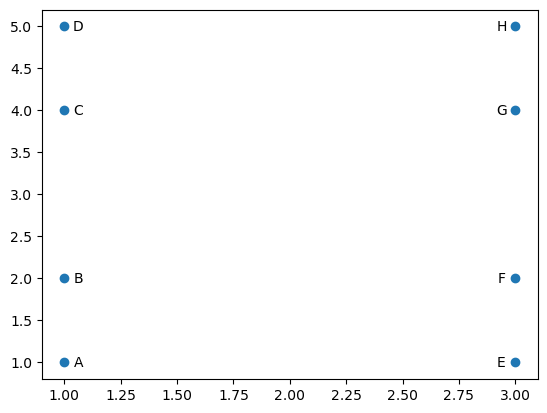
\includegraphics[width=0.7\textwidth]{scatter.png}
\end{center}
\subsection*{b.}
\label{sec:org102ca9a}
let's recompute the distance matrix for fun!
\begin{minted}[fontsize=\scriptsize]{python}
import scipy.cluster.hierarchy as shc
from scipy.spatial.distance import squareform, pdist


dist = pd.DataFrame(squareform(pdist(D[['x', 'y']]), 'euclidean'),
                    columns=D.index.values,
                    index=D.index.values)
dist
\end{minted}

\begin{verbatim}
          A         B         C         D         E         F         G  \
A  0.000000  1.000000  3.000000  4.000000  2.000000  2.236068  3.605551   
B  1.000000  0.000000  2.000000  3.000000  2.236068  2.000000  2.828427   
C  3.000000  2.000000  0.000000  1.000000  3.605551  2.828427  2.000000   
D  4.000000  3.000000  1.000000  0.000000  4.472136  3.605551  2.236068   
E  2.000000  2.236068  3.605551  4.472136  0.000000  1.000000  3.000000   
F  2.236068  2.000000  2.828427  3.605551  1.000000  0.000000  2.000000   
G  3.605551  2.828427  2.000000  2.236068  3.000000  2.000000  0.000000   
H  4.472136  3.605551  2.236068  2.000000  4.000000  3.000000  1.000000   

          H  
A  4.472136  
B  3.605551  
C  2.236068  
D  2.000000  
E  4.000000  
F  3.000000  
G  1.000000  
H  0.000000  
\end{verbatim}

This kind of clustering works by finding the closest euclidian points, merging
them into a cluster, then defining the distance to the cluster as the closest
point in the cluster. We'll use scipy to avoid the tedium.
\begin{minted}[fontsize=\scriptsize]{python}
fig, ax = plt.subplots()
dend = shc.dendrogram(shc.linkage(D[['x', 'y']], method='single'), labels=D.index, ax=ax)
plt.show()
\end{minted}

\begin{center}
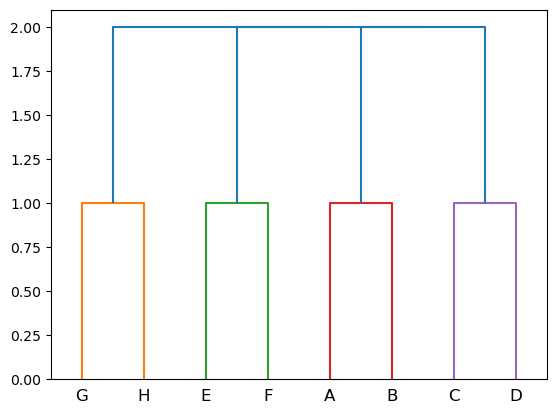
\includegraphics[width=0.7\textwidth]{./.ob-jupyter/9f5d3dc1356fe526c54aa18efddc8612d3017ce8.png}
\end{center}
\subsection*{c.}
\label{sec:orgcf9045b}

This kind of clustering works by finding the closest euclidian points, merging
them into a cluster, then defining the distance to the cluster as the farthest point
point in the cluster. We'll use scipy again to avoid the tedium.
\begin{minted}[fontsize=\scriptsize]{python}
fig, ax = plt.subplots()
dend = shc.dendrogram(shc.linkage(D[['x', 'y']], method='complete'), labels=D.index, ax=ax)
plt.show()
\end{minted}

\begin{center}
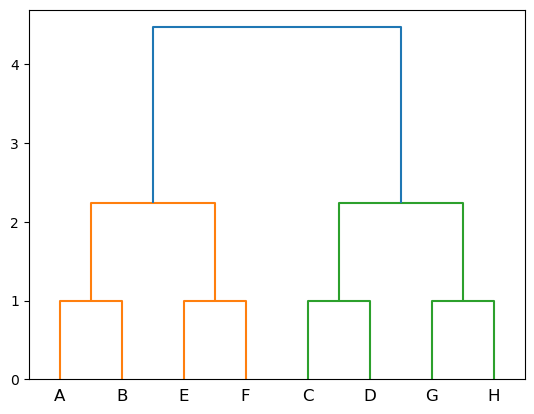
\includegraphics[width=0.7\textwidth]{./.ob-jupyter/32df2fc3bda014e92a08d750e03efcf510f513fa.png}
\end{center}
\end{document}